\documentclass[border=10pt]{standalone}
\usepackage{pgfplots}
\pgfplotsset{compat=1.17}
\begin{document}
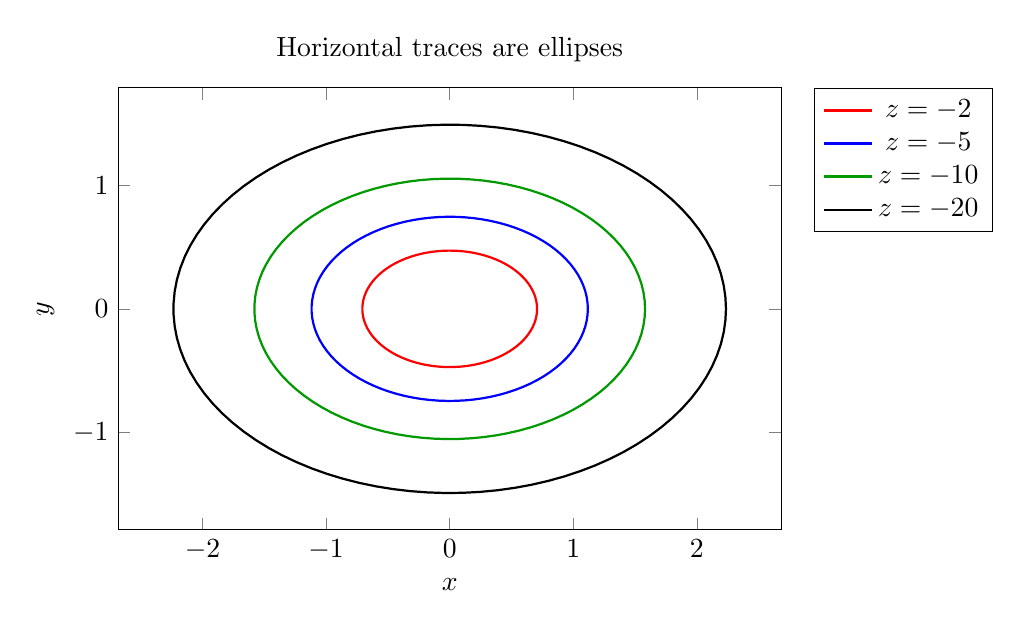
\begin{tikzpicture}
\begin{axis}[
    width=10cm,
    axis equal image,
    xlabel=$x$, ylabel=$y$,
    title={Horizontal traces are ellipses},
    legend style={at={(1.05,1)}, anchor=north west},
    domain=0:360,
    samples=100,
]
\addplot[red, thick, variable=\t] ({sqrt(2/4)*cos(\t)}, {sqrt(2/9)*sin(\t)});
\addlegendentry{$z=-2$}
\addplot[blue, thick, variable=\t] ({sqrt(5/4)*cos(\t)}, {sqrt(5/9)*sin(\t)});
\addlegendentry{$z=-5$}
\addplot[green!60!black, thick, variable=\t] ({sqrt(10/4)*cos(\t)}, {sqrt(10/9)*sin(\t)});
\addlegendentry{$z=-10$}
\addplot[black, thick, variable=\t] ({sqrt(20/4)*cos(\t)}, {sqrt(20/9)*sin(\t)});
\addlegendentry{$z=-20$}
\end{axis}
\end{tikzpicture}
\end{document}
